\documentclass{article}
  \usepackage[utf8]{inputenc}
  \usepackage[american]{babel}
  \usepackage{csquotes}
  \usepackage{hyperref}
  \usepackage[backend=biber,style=numeric,hyperref=true,natbib=true,autocite=plain,sorting=none]{biblatex}
  \usepackage[margin=1in]{geometry}
  \usepackage{fixltx2e}

  % this package and the below text is to force images to be added to the given section and subsection. See https://tex.stackexchange.com/questions/279/how-do-i-ensure-that-figures-appear-in-the-section-theyre-associated-with/235312#235312 for more information
  \usepackage{placeins}
  \let\Oldsection\section
  \renewcommand{\section}{\FloatBarrier\Oldsection}

  \let\Oldsubsection\subsection
  \renewcommand{\subsection}{\FloatBarrier\Oldsubsection}

  \let\Oldsubsubsection\subsubsection
  \renewcommand{\subsubsection}{\FloatBarrier\Oldsubsubsection}

  \addbibresource{references.bib}

  \title{%
    Image Processing Report: Web Image Filtering \\
    \large Stevens Institute of Technology}

  \date{December 11, 2018}
  \author{By Joshua Schmidt and Chris Blackwood}

  \usepackage{graphicx}

  \begin{document}

  \maketitle

  \bigskip
  \bigskip
  \bigskip
  \bigskip

  \begin{figure}[!htb]
    \centering
    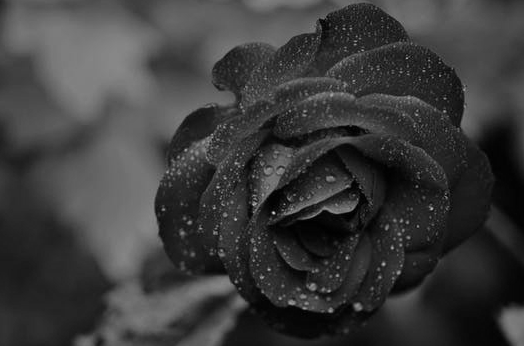
\includegraphics[width=0.75\textwidth]{assets/logo.png}
    \label{fig:logo}
  \end{figure}

  \newpage

  \tableofcontents

  \newpage

  % References to all attachments in the main body of the report

  \section{Abstract}

  The goal of this project was to create a web application with image processing capability, providing a suite for users to upload and modify images. Numerous image processing operations can be performed using this application, including Laplacian filters, histogram equalization, image sharpening, smoothing, negatives, vertical line detect, and more. Filters can be applied in succession to achieve an endless variety of results. The application is hosted online using the Firebase Development Platform, while most of the processing is performed locally on the client side. In effect, a rudimentary "Photoshop" tool has been successfully created.
  
  \newpage

  \section{Introduction}

  \subsection{Project objectives}

  The main objective of this project was to create a web application for the digital editing of photos in real-time.

  Key Project objectives included building an application utilizing industry-standard tools including JavaScript, jQuery, and Node.js. This project served as an ample opportunity to learn more about the best practices of web development, as well as using Git as a document management system. In order to maintain the large number of JavaScript files used for this project, the JavaScript management tool called Webpack was used to manage the files automatically.

  \subsection{Project Specifications}

  \subsubsection{Requirements}

  Minimum success criteria for this project included building an image processing tool capable of creating grayscale images, performing histogram equalization, creating negatives, and rudimentary line detection. No numerical success criteria were defined for this project; if this web application were been deployed in a commerical manner, it would be entirely necessary to define numerical criteria for image quality. However, being that mathemically deriving success criteria would likely take a disproportionate amount of time, it was decided that such a quality control process would be out of the scope of this project.
  
  As optional goals, a web application was to be created which could be hosted externally and accessed from anywhere within the world. Requirements for this application where that it needed to have adequate response time, loading in no more than 5 seconds (as user retention drops as page load times increase). Being a browser based application, this method of implementation allows for operating system cross compatibility, as users can upload images from smartphones, tablets, and desktop machines running any operating system of their choice.
  
  The second optional goal for this project was the addition of face detection algorithms to detect the presence of a face within an image based on rudimentary features using the WHAT ALGORITHM???. As machine learning is becoming a very commonly used technique in computer science, we may first think of solving this problem using machine learning to identify a face. However, using machine learning may introduce unnecesarry bugs into the system which are elusive to track down, thus reducing the reliability of the algorithm. Better practice in this case is to use the method that has the least opportunity for error, which would be feature detection. By programming in the particular features of interest, the programmer can have strict control over extraneous errors that would otherwise be introduced with a fast-and-loose method such as machine learning. However, due to time constraints as well as the additional complexity involved in the implementation of this algorithm, this part of the project was not completed.


  \subsection{Approach}

  Approach to project planning, scheduling, and completion.

  \begin{figure}[!htb]
    \centering
    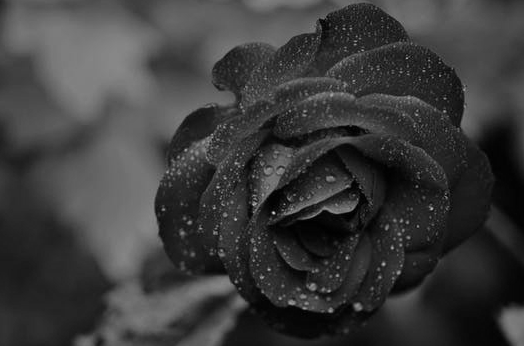
\includegraphics[width=0.75\textwidth]{assets/logo.png}
    \caption{scheduling chart}
    \label{fig:spacesuitdisplay}
  \end{figure}

  \newpage

  \section{Discussion}

  Once the project objectives were laid out, it was time to go about deciding on the implementation of the image filtering algorithms. It was known that the filters themselves would be fairly simple in design, as Laplacian operators, sharpening, smooth filters, and line detectors are fairly simple designs. Much of the thought spent on the design process involved the implementation of image processing itself.

  \subsection{Design}

  \subsubsection{Overview}

  In deciding upon the best means of implementing image processing algorithms, the team first considered the best means to bring this technology to the user. While MATLAB could have been used with great success, the team wished to create a more user-friendly tool which had greater cross-platform compatibility. MATLAB is only available on certain computers, and acquiring it requires a license. Rather than require users to download MATLAB and use our code, it was instead decided that the a more centralized approach could reach more users by using a server. Users could then interact with this central server, uploading images and selecting the algorithm to be performed on them. Being that the computational power necessary to perform these types of image processing is not particular intensive given today's powerful hardware, it was decided that JavaScript  could effectively be used to meet our requirements. 
  

  \subsubsection{Choice and Reasoning}

  Making a decision to use JavaScript as opposed to MATLAB depended upon numerous factors. While the project certaintly could have been completed with MATLAB, JavaScript, or even C++, there were numerous factors that made Javascript an attractive choice. The ability of the program to be run anywhere using only a web-enabled device was a huge advantage. In addition, having skills in creating web applications is very relevant in the tech economy of today; many software and hardware companies need web developers to develop their products or to provide secondary services that are associated with their hardware products. Internet of Things devices in particular make extensive use of web applications. It was thus decided that learning the use of JavaScript, Git, Node.js, and Webpack would prove invaluable skills in the marketplace. For this reason, the project was used as a learning experience for not only image processing, but the creation of web applications as well.

  \subsubsection{Design Analysis summary}

  Design analysis summary as developed from Truss Analyzer with interpretation of data

  \subsubsection{Fabrication}

  Fabrication concerns and considerations in the design phase

  \newpage

  \section{Conclusion and Recommendations}

  \subsection{Accomplishments}

  Describes the work in terms of accomplishments, both successful and unsuccessful

  \subsection{Recommendations}

  Provides recommendations to improve the project in terms of basic knowledge, materials, equipment, or other guidance

  Discuss what you would have done differently given the opportunity

  \newpage

  \section{Attachments}

  \subsection{Work Chart}

  Work break down structure and organization chart with roles and responsibilities

  \newpage

  \subsection{Truss Analysis}

  Truss Analysis jpg and csv printouts for final truss design

  \newpage

  \subsection{Alternatives Truss Analysis}

  Truss Analysis jpg and csv printouts for at least two alternate designs considered

  \newpage

  \subsection{Data}

  Brass compression data, charts, and formulas

  \newpage

  \printbibliography

  \end{document}
